%% LyX 2.5.1 created this file.  For more info, see https://www.lyx.org/.
%% Do not edit unless you really know what you are doing.
\documentclass[brazil]{article}
\usepackage[T1]{fontenc}
\usepackage[utf8]{inputenc}
\usepackage{babel}
\usepackage{mathtools}
\usepackage{amsmath}
\usepackage{graphicx}
\usepackage{geometry}
\geometry{verbose,tmargin=3cm,bmargin=3cm,lmargin=3cm,rmargin=2.5cm}
\usepackage[]
 {hyperref}
\begin{document}
\title{Descrição da dinâmica da riqueza via Fokker-Planck}

\maketitle
Eu sempre quis abordar a questão da distribuição de riqueza sob a perspectiva de processos de Markov e afins e é isso que vou fazer através do artigo ``Fokker-Planck Description of Wealth Dynamics and the Origin of Pareto's Law'' \cite{boghosian2014a}.

Vamos lembrar que obtivemos, para uma variável, a equação
\begin{align*}
\frac{\partial P\left(x,t\right)}{\partial t} & =\frac{\partial^{2}}{\partial x^{2}}\left[DP\left(x,t\right)\right]+\frac{\partial}{\partial x}\left[D\beta\frac{\partial U\left(x\right)}{\partial x}P\left(x,t\right)\right]
\end{align*}

Neste caso, assumimos um coeficiente de difusão constante, ($A=D$), e uma deriva determinada por um potencial conservativo, ($C=D\beta\frac{\partial U\left(x\right)}{\partial x}$). De forma mais geral, a equação pode ser escrita como:

\begin{align*}
\frac{\partial P}{\partial t} & =\frac{\partial^{2}}{\partial x^{2}}\left[A\left(x\right)P\right]+\frac{\partial}{\partial x}\left[B\left(x\right)P\right]
\end{align*}

Ou seja, em uma dimensão, a evolução temporal da densidade de probabilidade é determinada pela derivada espacial de dois fluxos: um fluxo difusivo, associado às flutuações aleatórias, e um fluxo de deriva, associado à tendência determinística imposta pelas forças externas.

Quando $x$ varia em pequenos passos estocáticos $\Delta x$, queremos então o coeficiente de difusão $A=\frac{1}{2}\left\langle \Delta x^{2}\right\rangle $ e a deriva $B=\left\langle \Delta x\right\rangle $\footnote{Na literatura tipicamente vamos encontrar $\dot{P}(\mathbf{r},t)=\frac{1}{2}\nabla^{2}\boldsymbol{D}P-\nabla\cdot\left(\boldsymbol{C}P\right)$. Além disso podemos escrever como $\dot{P}(\mathbf{r},t)=\nabla\cdot\boldsymbol{A}\left(\mathbf{r},t\right)+\nabla\cdot\boldsymbol{B}\left(\mathbf{r},t\right)$, ou seja, temos a a evolução temporal da probabilidade dada pela divergência da soma de dois fluxos: um difusivo e outro devido à força externa.}.

Mas antes de avançar, vamos buscar entender como essa equaçaõ foi obtida.

\subsection{Equação de Fokker-Planck com passos de pequena variação}

Esta dedução é baseada no trabaho do professor Heff Moehlis ``Derivation of the Fokker-Planck Equation''\cite{MoehlisAppendixFokkerPlanck}. Vamos denotar $\left\{ X\left(t\right):t\geq0\right\} $um processo estocástico unidimensional com $t_{1}>t_{2}>t_{3}$, ou seja, opost do habitual. Se $t_{2}$ é o presente, então $t_{1}$é o futuro e $t_{3}$ o passado.
\begin{itemize}
\item $P\left(X_{1},t_{1};X_{2},t_{2}\right)$é a probabilidade de que $X\left(t_{1}\right)=X$ e $X\left(t_{2}\right)=X_{2}$ (distribuição de probabilidade conjunta).
\item P$\left(X_{1},t_{1}|X_{2},t_{2}\right)$ é a probabilidade que $X\left(t_{1}\right)=X_{1}$ dado que $X\left(t_{2}\right)=X_{2}$ (probabilidade de transição)
\end{itemize}
Temos então:

\[
P\left(X_{1},t_{1};X_{2},t_{2}\right)=P\left(X_{1},t_{1}|X_{2},t_{2}\right)P\left(X_{2},t_{2}\right)
\]

A probabilidade conjunta de o sistema estar no estado $X_{2}$ no instante $t_{2}$ e no estado $X_{1}$ no instante posterior $t_{1}$ é igual ao produto da probabilidade de o sistema estar em $X_{2}$ no instante $t_{2}$ pela probabilidade condicional de que, estando em $X_{2}$ em $t_{2}$, ele evolua para o estado $X_{1}$ no instante $t_{1}$\footnote{Isso é a probabilidade conjunta $P\left(A\cap B\right)=P\left(A|B\right)P\left(B\right).$}.

Vamos assumir que $X\left(t\right)$é um processo de Markov:

\[
P\left(X_{1},t_{1}|X_{2},t_{2};X_{3},t_{3}\right)=P\left(X_{1},t_{1}|X_{2},t_{2}\right)
\]

Ou seja, a probabilidade do sistema transicionar para o estado $X_{1}$, depende apenas do seu estado imediatamente anterior $X_{2}$, a inforção quanto aos outros estados anteriores naõ agrega nova informaçao. Para um processo de Markov, a seguinte equação de Chapman-Kolmoforov é satisfeita:

\[
P\left(X_{1},t_{1}|X_{3},t_{3}\right)=\int P\left(X_{1},t_{1}|X_{2},t_{2}\right)P\left(X_{2},t_{2}|X_{3},t_{3}\right)dX_{2}
\]

A equação de Chapman-Kolmogorov estabelece que a probabilidade de o sistema evoluir do estado $X_{3}$ no instante $t_{3}$ para o estado $X_{1}$ no instante $t_{1}$ pode ser obtida considerando todos os estados intermediários possíveis $X_{2}$ no instante $t_{2}$. Para cada estado intermediário, multiplica-se a probabilidade de o sistema evoluir de $X_{3}$ para $X_{2}$ pela probabilidade de evoluir de $X_{2}$ para $X_{1}$ e, em seguida, integra-se sobre todos os valores possíveis de $X_{2}$, isto é, sobre todos possíveis estados intermediários.

Vamos considerar que as probabilidades de transição não dependem do tempo absoluto, apenas do intervalo de tempo transcorrido. Então por simplicidade na notação $P\left(X_{1},t_{1}-t_{2}|X_{2}\right)\equiv P\left(X_{1},t_{1}|X_{2},t_{2}\right).$ Escrevendo então $P\left(Y,t|X\right)\equiv P\left(Y,t|X,0\right)$, ou seja, temos $X\left(0\right)=Y$ e $X\left(t\right)=X$. Vamos começar considerando:

\[
\int h\left(Y\right)\frac{\partial P\left(Y,t|X\right)}{\partial t}dY=I
\]

Onde $h\left(Y\right)$ possui um intervalo finito $Y\in\left[a,b\right]$ onde para todo $Y$ fora deste intervalo, temos $h\left(Y\right)=0$\footnote{Aparentemente é isso que o artigo quer dizer com ``compact support''.}. Escrevendo:

\[
\frac{\partial P\left(Y,t|X\right)}{\partial t}=\lim_{\Delta t\rightarrow0}\frac{P\left(Y,t+\Delta t|X\right)-P\left(Y,t|X\right)}{\Delta t}
\]

Substituindo na Integral, e usando a equação de Chapman-Kolmogorov 

\begin{align*}
I & =\lim_{\Delta t\rightarrow0}\int h\left(Y\right)\frac{P\left(Y,t+\Delta t|X\right)-P\left(Y,t|X\right)}{\Delta t}dY\\
 & =\lim_{\Delta t\rightarrow0}\frac{1}{\Delta t}\left[\int h\left(Y\right)P\left(Y,t+\Delta t|X\right)dY-\int h\left(Y\right)P\left(Y,t|X\right)dY\right]\\
 & =\lim_{\Delta t\rightarrow0}\frac{1}{\Delta t}\left[\int h\left(Y\right)\left(\int P\left(Y,\Delta t|Z\right)P\left(Z,t|X\right)dZ\right)dY-\int h\left(Y\right)P\left(Y,t|X\right)dY\right]
\end{align*}

Ou seja, inicialmente tínhamos apenas uma transição direta de $X$ para $Y$, separada por um intervalo de tempo $t+\Delta t$. Ao aplicar a equação de Chapman-Kolmogorov, introduzimos um estado intermediário $Z$ no instante $t$, decompondo a trajetória em duas transições sucessivas. A primeira descreve a evolução de $X$ até $Z$, cujo intervalo de tempo é $t-0=t$, enquanto a segunda descreve a evolução de $Z$ até $Y$, cujo intervalo é $(t+\Delta t)-t=\Delta t$. Como o processo é homogêneo no tempo, a probabilidade de transição depende apenas da duração do intervalo e não do instante absoluto em que ele ocorre. Assim, $P\left(Y,t+\Delta t\mid Z,t\right)=P\left(Y,\Delta t\mid Z\right).$ Note que apenas a segunda transição é reescrita dessa forma; o intervalo total entre $X$ e $Y$ continua sendo $t+\Delta t$.

Como a integral percorre todos os possíveis estados, a variável de integração não representa um estado específico, mas apenas um índice que enumera todos os estados possíveis. Por isso podemos trocar $Y$ por $Z$ (ou por qualquer outra letra), desde que a troca seja feita de forma consistente em toda a integral. Então podemos reescrever a integral sobre $dY$ como por $dZ$ na segunda integral:

\begin{align*}
I & =\lim_{\Delta t\rightarrow0}\frac{1}{\Delta x}\left[\int h\left(Y\right)\left(\int P\left(Y,\Delta t|Z\right)P\left(Z,t|X\right)dZ\right)dY-\int h\left(Z\right)P\left(Z,t|X\right)dZ\right]\\
 & =\lim_{\Delta t\rightarrow0}\frac{1}{\Delta x}\left[\int P\left(Z,t|X\right)\left(\int h\left(Y\right)P\left(Y,\Delta t|Z\right)dY-h\left(Z\right)\right)dZ\right]\\
 & =
\end{align*}

E como $\int^{+\infty}_{-\infty}P\left(Y,\Delta t|Z\right)dY=1$, afinal tem 100\% de chnce do sistema ir do estado $Z$ para algum estado qualquer (estamos integrando sobre todos estados possíveis), e como $h\left(Z\right)$ não depende de $Y$, $h\left(Z\right)\int f\left(Y\right)dY=\int h\left(Z\right)f\left(Y\right)dY$ então:

\begin{align*}
I & =\lim_{\Delta t\rightarrow0}\frac{1}{\Delta t}\left[\int P\left(Z,t|X\right)\left(\int h\left(Y\right)P\left(Y,\Delta t|Z\right)dY-\int h\left(Z\right)P\left(Y,\Delta t|Z\right)dY\right)dZ\right]\\
 & =\lim_{\Delta t\rightarrow0}\frac{1}{\Delta t}\left[\int P\left(Z,t|X\right)\int P\left(Y,\Delta t|Z\right)\left(h\left(Y\right)-h\left(Z\right)\right)dYdZ\right]
\end{align*}

Fazendo então uma expansão em série de taylor de $h\left(Y\right)$em torno de $Z$:

\begin{align*}
h\left(Y\right) & =\sum^{\infty}_{n=0}\frac{h^{\left(n\right)}\left(Z\right)}{n!}\left(Y-Z\right)^{n}=h\left(Z\right)+\sum^{\infty}_{n=1}\frac{h^{\left(n\right)}\left(Z\right)}{n!}\left(Y-Z\right)^{n}
\end{align*}

\begin{align*}
I & =\lim_{\Delta t\rightarrow0}\frac{1}{\Delta t}\left[\int P\left(Z,t|X\right)\int P\left(Y,\Delta t|Z\right)\left(h\left(Z\right)+\sum^{\infty}_{n=1}\frac{h^{\left(n\right)}\left(Z\right)}{n!}\left(Y-Z\right)^{n}-h\left(Z\right)\right)dYdZ\right]\\
 & =\int P\left(Z,t|X\right)\sum^{\infty}_{n=0}\left[\frac{1}{n!}\lim_{\Delta t\rightarrow0}\frac{1}{\Delta t}\int P\left(Y,\Delta t|Z\right)\left(Y-Z\right)^{n}dY\right]h^{\left(n\right)}\left(Z\right)dZ
\end{align*}

Definindo os momentos de salto como:

\[
D^{\left(n\right)}\left(Z\right)=\frac{1}{n!}\lim_{\Delta t\rightarrow0}\frac{1}{\Delta t}\int\left(Y-Z\right)^{n}P\left(Y,\Delta t|Z\right)dY
\]

Para entender a ideia de salto, podemos lembrar que $X\left(t+\Delta t\right)-X\left(t\right)=Y-Z$. Ficamos então com:

\begin{align*}
\int h\left(Y\right)\frac{\partial P\left(Y,t|X\right)}{\partial t}dY & =\sum^{\infty}_{n=1}\int P\left(Z,t|X\right)D^{\left(n\right)}h^{\left(n\right)}\left(Z\right)dZ
\end{align*}

Então cada termo da soma é:

\[
\int P\left(Z,t|X\right)D^{\left(n\right)}h^{\left(n\right)}\left(Z\right)dZ=\int F_{n}\left(Z\right)h^{\left(n\right)}\left(Z\right)dZ
\]

Sendo $F_{n}\left(Z\right)=P\left(Z,t|X\right)D^{\left(n\right)}$. Para $n=1$, aplicando integral por partes então fazendo $u=F_{1}\left(Z\right)=P\left(Z,t|X\right)D^{\left(1\right)}$ ($du=F^{\left(1\right)}_{1}dZ$) e $dv=h^{\left(1\right)}\left(Z\right)dZ$ ($v=h\left(Z\right)$)

\begin{align*}
\int udv & =uv-\int vdu\\
\int^{+\infty}_{-\infty}F_{1}\left(Z\right)h^{\left(1\right)}\left(Z\right)dZ & =\left[h\left(Z\right)F_{1}\left(Z\right)\right]^{+\infty}_{-\infty}-\int^{+\infty}_{-\infty}h\left(Z\right)F^{\left(1\right)}_{1}dZ
\end{align*}

Como a função teste $h(Z)$ possui suporte compacto, o termo de contorno desaparece, já que ele é zero fora da reggião de interesse. Então temos apenas:

\begin{align*}
\int^{+\infty}_{-\infty}F_{1}\left(Z\right)h^{\left(1\right)}\left(Z\right)dZ & =-\int^{+\infty}_{-\infty}h\left(Z\right)F^{\left(1\right)}_{1}dZ
\end{align*}

Pra $n=2$, aplicando integral por partes então fazendo $u=F_{2}\left(Z\right)=P\left(Z,t|X\right)D^{\left(2\right)}$ ($du=F^{\left(1\right)}_{2}dZ$) e $dv=h^{\left(2\right)}\left(Z\right)dZ$ ($v=h^{\left(1\right)}\left(Z\right)$).

\begin{align*}
\int^{+\infty}_{-\infty}F_{2}\left(Z\right)h^{\left(2\right)}\left(Z\right)dZ & =-\int^{+\infty}_{-\infty}h^{\left(1\right)}F^{\left(1\right)}_{2}dZ
\end{align*}

Novamente, devido ao fato de $h(Z)$ possuir suporte compacto, temos que $h'(Z)=0$ fora do seu suporte, isto é, nas extremidades do domínio de integração.. E fazend novamente uma integral por partes sendo $u=F^{\left(1\right)}_{2}=P\left(Z,t|X\right)D^{\left(2\right)}$ ($du=F^{\left(2\right)}_{2}dZ$) e $dv=h^{\left(1\right)}\left(Z\right)dZ$ ($v=h\left(Z\right)$). Então:

\begin{align*}
\int^{+\infty}_{-\infty}F_{2}\left(Z\right)h^{\left(2\right)}\left(Z\right)dZ & =\int^{+\infty}_{-\infty}hF^{\left(2\right)}_{2}dZ
\end{align*}

Então de forma geral temos:

\begin{align*}
\int F_{n}\left(Z\right)h^{\left(n\right)}\left(Z\right)dZ & =\left(-1\right)^{n}\int h\left(Z\right)F^{\left(n\right)}_{n}dZ\\
 & =\int h\left(Z\right)\left(-\frac{\partial}{\partial Z}\right)^{n}P\left(Z,t|X\right)D^{\left(n\right)}dZ
\end{align*}

Então:

\begin{align*}
\int h\left(Y\right)\frac{\partial P\left(Y,t|X\right)}{\partial t}dY & =\sum^{\infty}_{n=1}\int P\left(Z,t|X\right)D^{\left(n\right)}h^{\left(n\right)}\left(Z\right)dZ\\
 & =\int h\left(Z\right)\sum^{\infty}_{n=1}\left(-\frac{\partial}{\partial Z}\right)^{n}D^{\left(n\right)}P\left(Z,t|X\right)dZ
\end{align*}

Passando o lado esquerdo pro direito e novamente $Y\rightarrow Z$ na esquerda:

\begin{align*}
\int h\left(Z\right)\frac{\partial P\left(Z,t|X\right)}{\partial t}dZ-\int h\left(Z\right)\sum^{\infty}_{n=1}\left(-\frac{\partial}{\partial Z}\right)^{n}D^{\left(n\right)}P\left(Z,t|X\right)dZ & =0\\
\int h\left(Z\right)\left(\frac{\partial P\left(Z,t|X\right)}{\partial t}-\sum^{\infty}_{n=1}\left(-\frac{\partial}{\partial Z}\right)^{n}D^{\left(n\right)}P\left(Z,t|X\right)\right)dZ & =0
\end{align*}

Como $h\left(Z\right)$ é uma funçaõ arbitrária, para garantir que essa integral seja zero, precisamos que:

\[
\frac{\partial P\left(Z,t|X\right)}{\partial t}-\sum^{\infty}_{n=1}\left(-\frac{\partial}{\partial Z}\right)^{n}D^{\left(n\right)}P\left(Z,t|X\right)=0
\]

Escrevendo $P\left(X,t\right)\equiv P\left(X,t|X_{0},0\right)$, ou seja, esta é a probabilidade (densidade) de encontrar o sistema no estado $X$ no instante $t$, dado que ele estava no estado $X_{0}$ no instante 0. Então:

\[
\frac{\partial P\left(X,t\right)}{\partial t}-\sum^{\infty}_{n=1}\left(-\frac{\partial}{\partial X}\right)^{n}D^{\left(n\right)}P\left(X,t\right)=0
\]

E tendo uma uma distribuição $\delta$ como condição inical e $X_{0}$ Então a probabilidade de obtermos $X$ no instante $0$ é $P\left(X,0\right)=\delta\left(X-X_{0}\right)$, isto significa que, no instante inicial, a variável aleatória $X$ assume o valor $X_{0}$ com probabilidade unitária. Toda a distribuição de probabilidade está concentrada em $X_{0}$, sendo representada pela distribuição delta de Dirac. Temos então para $D^{\left(n\right)}$:

\begin{align*}
D^{\left(n\right)}\left(Z\right) & =\frac{1}{n!}\lim_{\Delta t\rightarrow0}\frac{1}{\Delta t}\int\left(Y-Z\right)^{n}P\left(Y,\Delta t|Z\right)dY\\
D^{\left(n\right)}\left(X_{0}\right) & =\frac{1}{n!}\lim_{\Delta t\rightarrow0}\frac{1}{\Delta t}\int\left(X-X_{0}\right)^{n}P\left(X,\Delta t|X_{0}\right)dX\\
 & =\frac{1}{n!}\lim_{\Delta t\rightarrow0}\frac{1}{\Delta t}\int\left(\Delta X\right)^{n}P\left(X,\Delta t|X_{0}\right)dX
\end{align*}

E pela definição de valores médios:

\[
D^{\left(n\right)}\left(X_{0}\right)=\frac{1}{n!}\lim_{\Delta t\rightarrow0}\frac{\left\langle \left(\Delta X\right)^{n}\right\rangle }{\Delta t}
\]

Onde $\left\langle (\Delta X)^{n}\right\rangle $ representa o valor esperado de$(\Delta X)^{n}$, com $\Delta X=X\left(\Delta t\right)-X_{0}\left(0\right)$, calculado em relação à distribuição de transição, isto é, considerando todas as possíveis transições do estado $X_{0}$, no instante $0$, para os estados $X$, no instante $\Delta t$. Considerando que $D^{\left(n\right)}\left(X\right)=0$ para $n>2$ então:

\begin{align*}
\frac{\partial P\left(X,t\right)}{\partial t}+\frac{\partial}{\partial X}\left[D^{\left(1\right)}P\left(X,t\right)\right]-\left(\frac{\partial}{\partial X}\right)^{2}D^{\left(2\right)}P\left(X,t\right) & =0
\end{align*}

Para $n=1$ e $n=2$:
\[
D^{\left(1\right)}\left(X_{0}\right)=\lim_{\Delta t\rightarrow0}\frac{\left\langle \Delta X\right\rangle }{\Delta t},\quad D^{\left(2\right)}\left(X_{0}\right)=\frac{1}{2}\lim_{\Delta t\rightarrow0}\frac{\left\langle \left(\Delta X\right)^{2}\right\rangle }{\Delta t}
\]

Então:

\begin{align*}
\frac{\partial P\left(X,t\right)}{\partial t} & =-\frac{\partial}{\partial X}\left[\lim_{\Delta t\rightarrow0}\frac{\left\langle \Delta X\right\rangle }{\Delta t}P\left(X,t\right)\right]+\frac{\partial^{2}}{\partial X^{2}}\left[\frac{1}{2}\lim_{\Delta t\rightarrow0}\frac{\left\langle \left(\Delta X\right)^{2}\right\rangle }{\Delta t}P\left(X,t\right)\right]\\
 & =-\frac{\partial}{\partial X}\left[V\left(X\right)P\left(X,t\right)\right]+\frac{\partial^{2}}{\partial X^{2}}\left[D\left(X\right)P\left(X,t\right)\right]
\end{align*}

Onde o primeiro termo $V\left(X\right)\equiv D^{\left(1\right)}\left(X\right)$ é o coeficiente de deriva. Sendo:

\[
D^{\left(1\right)}\left(X_{0}\right)=\lim_{\Delta t\rightarrow0}\frac{\left\langle \Delta X\right\rangle }{\Delta t}=\left.\lim_{\Delta t\rightarrow0}\frac{\left\langle X\left(t+\Delta t\right)\right\rangle -\left\langle X\left(t\right)\right\rangle }{\Delta t}\right|_{t=0}=\left.\frac{\partial\left\langle X\right\rangle }{\partial t}\right|_{t=0}
\]

E $D\left(X\right)\equiv D^{\left(2\right)}\left(X\right)$ é o coeficiente de difusão. Lembrando que com:

\[
\begin{array}{c}
\left.\left\langle \Delta X\right\rangle \right|_{t=0}=\left.\left\langle X\left(t+\Delta t\right)\right\rangle -\left\langle X\left(t\right)\right\rangle \right|_{t=0}=\left\langle X\left(\Delta t\right)\right\rangle -\left\langle X\left(0\right)\right\rangle =\left\langle X\left(\Delta t\right)\right\rangle -\left\langle X_{0}\right\rangle \\
\left.X\left(\Delta t\right)\right|_{t=0}=\left.\Delta X\right|_{t=0}+X_{0}
\end{array}
\]

Uma vez que $\left\langle X_{0}\right\rangle =X_{0}$ é uma constante, por conveonção vamos parar de indicar que estamos avaliando em $t=0$, mas isso deve ficar subentendido. Então se a variância no instante $t$ tendo $X_{0}$ como estado inicial é dado por:

\begin{align*}
\sigma^{2}\left(\Delta t;X_{0}\right) & =\left\langle X\left(\Delta t\right)^{2}\right\rangle -\left\langle X\left(\Delta t\right)\right\rangle ^{2}\\
 & =\left\langle \left(\Delta X+X_{0}\right)^{2}\right\rangle -\left\langle \Delta X+X_{0}\right\rangle ^{2}\\
 & =\left\langle \Delta X^{2}+X^{2}_{0}+2X_{0}\Delta X\right\rangle -\left(X_{0}+\left\langle \Delta X\right\rangle \right)^{2}\\
 & =\left\langle \Delta X^{2}\right\rangle +X^{2}_{0}+2X_{0}\left\langle \Delta X\right\rangle -\left(\left\langle \Delta X\right\rangle ^{2}+X^{2}_{0}+2X_{0}\left\langle \Delta X\right\rangle \right)\\
 & =\left\langle \Delta X^{2}\right\rangle -\left\langle \Delta X\right\rangle ^{2}\\
\left\langle \Delta X^{2}\right\rangle  & =\sigma^{2}\left(\Delta t;X_{0}\right)+\left\langle \Delta X\right\rangle ^{2}
\end{align*}

Então:

\begin{align*}
D^{\left(2\right)}\left(X_{0}\right) & =\frac{1}{2}\lim_{\Delta t\rightarrow0}\frac{\left\langle \left(\Delta X\right)^{2}\right\rangle }{\Delta t}\\
 & =\frac{1}{2}\lim_{\Delta t\rightarrow0}\frac{\sigma^{2}\left(\Delta t;X_{0}\right)+\left\langle \Delta X\right\rangle ^{2}}{\Delta t}\\
 & =\frac{1}{2}\lim_{\Delta t\rightarrow0}\frac{\sigma^{2}\left(\Delta t;X_{0}\right)}{\Delta t}+\frac{1}{2}\lim_{\Delta t\rightarrow0}\frac{\left\langle \Delta X\right\rangle ^{2}}{\Delta t}
\end{align*}

Agora, quanto ao primeiro momento, tínhamos $D^{(1)}(X_{0})=\lim_{\Delta t\rightarrow0}\frac{\langle\Delta X\rangle}{\Delta t}$. Para um intervalo de tempo suficientemente pequeno, podemos aproximar $D^{(1)}(X_{0})\approx\frac{\langle\Delta X\rangle}{\Delta t}$ , ou, de forma equivalente, $\langle\Delta X\rangle\approx D^{(1)}(X_{0})\Delta t$. Então para o segundo termo:

\[
\lim_{\Delta t\rightarrow0}\frac{\left\langle \Delta X\right\rangle ^{2}}{\Delta t}=\lim_{\Delta t\rightarrow0}\frac{\left[D^{(1)}(X_{0})\right]^{2}\Delta t^{2}}{\Delta t}=\lim_{\Delta t\rightarrow0}\left[D^{(1)}(X_{0})\right]^{2}\Delta t=\left[D^{(1)}(X_{0})\right]^{2}\lim_{\Delta t\rightarrow0}\Delta t=0
\]

Agora resta o primeiro termo. Se:

\[
\left.\frac{\partial\sigma^{2}}{\partial t}\right|_{t=0}=\left.\lim_{\Delta t\rightarrow0}\frac{\sigma^{2}\left(t+\Delta t;X_{0}\right)-\sigma^{2}\left(t;X_{0}\right)}{\Delta t}\right|_{t=0}=\lim_{\Delta t\rightarrow0}\frac{\sigma^{2}\left(\Delta t;X_{0}\right)-\sigma^{2}\left(0;X_{0}\right)}{\Delta t}=\lim_{\Delta t\rightarrow0}\frac{\sigma^{2}\left(\Delta t;X_{0}\right)}{\Delta t}
\]

Uma vez que a variância no instante inicial é nula $\sigma^{2}\left(0;X_{0}\right)$, isto é, sabemos o valor com exatidão. Então:

\begin{align*}
D^{\left(2\right)}\left(X_{0}\right) & =\frac{1}{2}\left.\frac{\partial\sigma^{2}}{\partial t}\right|_{t=0}
\end{align*}

Ou seja, temos:

\begin{align*}
\frac{\partial P\left(X,t\right)}{\partial t} & =-\frac{\partial}{\partial X}\left[V\left(X\right)P\left(X,t\right)\right]+\frac{\partial^{2}}{\partial X^{2}}\left[D\left(X\right)P\left(X,t\right)\right]
\end{align*}

Com:

\[
V\left(X_{0}\right)=\left.\frac{\partial\left\langle X\left(t;X_{0}\right)\right\rangle }{\partial t}\right|_{t=0}\qquad D\left(X_{0}\right)=D^{\left(2\right)}\left(X_{0}\right)=\frac{1}{2}\left.\frac{\partial\sigma\left(t;X_{0}\right)^{2}}{\partial t}\right|_{t=0}
\]


\subsection{O modelo Yard-Sale}

Ou seja, sendo $x=w$ obtemos a equação do artigo:

\begin{align*}
\frac{\partial P}{\partial t} & =-\frac{\partial}{\partial w}\left[\lim_{\Delta t\rightarrow0}\frac{\left\langle \Delta w\right\rangle }{\Delta t}P\right]+\frac{\partial^{2}}{\partial w^{2}}\left[\frac{1}{2}\lim_{\Delta t\rightarrow0}\frac{\left\langle \Delta w\Delta w\right\rangle }{\Delta t}P\right]
\end{align*}

E no artigo temos:

\begin{align*}
\frac{\partial P}{\partial t} & =-\frac{\partial}{\partial w}\left[\left\langle \Delta\left(w\right)\right\rangle P\right]+\frac{\partial^{2}}{\partial w^{2}}\left[\frac{1}{2}\left\langle \Delta\left(w\right)\Delta\left(w\right)\right\rangle P\right]
\end{align*}

Ou seja:

\[
\left\langle \Delta\left(w\right)\right\rangle =\lim_{\Delta t\rightarrow0}\frac{\left\langle \Delta w\right\rangle }{\Delta t}\qquad\left\langle \Delta\left(w\right)^{2}\right\rangle =\lim_{\Delta t\rightarrow0}\frac{\left\langle \left(\Delta w\right)^{2}\right\rangle }{\Delta t}
\]

Para demonstrar essa relação, introduzimos algumas hipóteses adicionais. Considere uma única realização do processo durante um intervalo de tempo $\Delta t$, no qual ocorrem$\Delta N$ transações e a riqueza total transferida é $\Delta w$. Definimos a riqueza média transferida por transação nessa realização como

\[
\left\langle \Delta(w)_{1}\right\rangle \equiv\frac{\Delta w}{\Delta N},
\]

de onde segue imediatamente que

\[
\Delta w=\Delta N\left\langle \Delta(w)_{1}\right\rangle .
\]

Em seguida, generalizamos para um ensemble de realizações, nas quais tanto $\Delta w$ quanto $\Delta N$ podem variar. Tomando a esperança matemática sobre esse ensemble e assumindo que o número de transações ocorridas em um intervalo é estatisticamente independente da riqueza média transferida por transação, obtemos\footnote{A mudança de notação $\left\langle \Delta\left(w\right)_{1}\right\rangle \rightarrow\left\langle \Delta\left(w\right)\right\rangle $ indoca que agora não é mais a média dentro de uma única realização, mas sobre o ensemble.}

\[
\left\langle \Delta w\right\rangle =\left\langle \Delta N\right\rangle \left\langle \Delta(w)\right\rangle .
\]

Como processo de Poison consideramos que a probabilidade de um evento acontecer em um intervalo de tempo pequeno, é proporcional ao tempo. Ou seja $\left\langle \Delta N\right\rangle =\lambda\Delta t$, quanto maior o intervalo, maior a probabilidade que uma troca ocorra.

\begin{align*}
\left\langle \Delta w\right\rangle = & \left\langle \Delta N\right\rangle \left\langle \Delta\left(w\right)\right\rangle \\
\left\langle \Delta w\right\rangle = & \lambda\Delta t\left\langle \Delta\left(w\right)\right\rangle \\
\frac{\left\langle \Delta w\right\rangle }{\Delta t}= & \lambda\left\langle \Delta\left(w\right)\right\rangle 
\end{align*}

Escolheremos então a unidade de tempo de forma que o tempo médio entre transações seja unitário. Nessa escala, a taxa de transações é $\lambda=1$ de modo que $\left\langle \Delta N\right\rangle =\Delta t$, ou seja, há em média uma transação por unidade de tempo. Então:

\[
\frac{\left\langle \Delta w\right\rangle }{\Delta t}=\left\langle \Delta\left(w\right)\right\rangle \rightarrow\lim_{\Delta t\rightarrow0}\frac{\left\langle \Delta w\right\rangle }{\Delta t}=\left\langle \Delta\left(w\right)\right\rangle 
\]

Uma vez que o lado direito não depende de $\Delta t$. Raciocínio análogo se aplica a $\left\langle \Delta\left(w\right)^{2}\right\rangle $. Mas vamos dar um passo anterior a $\left\langle \Delta(w)_{1}\right\rangle \equiv\frac{\Delta w}{\Delta N}$ e reforçar a hipótese de trabalharmos com um processo de Poisson. Considere uma única realização do processo durante um intervalo de tempo $\Delta t$, no qual ocorrem $\Delta N$ transações:

\begin{align*}
\Delta w & =\sum^{\Delta N}_{i=1}\Delta(w)_{i}\\
\left(\Delta w\right)^{2} & =\sum^{\Delta N}_{i,j=1}\Delta(w)_{i}\Delta(w)_{j}\\
 & =\sum^{\Delta N}_{i=1}\Delta(w)^{2}_{i}+\left(\sum^{\Delta N}_{i\neq j}\Delta(w)_{j}\Delta(w)_{i}\right)\\
\left\langle \left(\Delta w\right)^{2}\right\rangle  & =\left\langle \Delta N\right\rangle \left\langle \Delta(w)^{2}_{E}\right\rangle +\left\langle \sum^{\Delta N}_{i\neq j}\Delta(w)_{j}\Delta(w)_{i}\right\rangle 
\end{align*}

Para o primeiro termo repetimos a argumentação do caso anterior. Como evitamos $i=j$, se no primeiro somatório temos $\Delta N$ termos, no segundo somamos sobre $\Delta N$ para $i$ e $\Delta N-1$ para $j$ por exemplo, evitando quando $i\neq j$. Assim o segundo somatório se dá por $\Delta N\left(\Delta N-1\right)$ termos. Denotando uma média sobre o ensemble dos termos $\left\langle \Delta(w)_{j}\Delta(w)_{i}\right\rangle$   por $\left\langle \Delta\Delta(w)_{E}\right\rangle $, escrevemos:

\begin{align*}
\left\langle \left(\Delta w\right)^{2}\right\rangle  & =\left\langle \Delta N\right\rangle \left\langle \Delta(w)^{2}_{E}\right\rangle +\left\langle \Delta N\left(\Delta N-1\right)\right\rangle \left\langle \Delta\Delta(w)_{E}\right\rangle 
\end{align*}

Porém agora$\left\langle \Delta N\left(\Delta N-1\right)\right\rangle $ é um pouco mais complicado que $\left\langle \Delta N\right\rangle =\lambda\Delta t$. Por hora vamos utilizar o momento fatorial de Poisson (\href{https://en.wikipedia.org/wiki/Factorial_moment_generating_function}{Wikipedia}). Utilizando a notação $\left(x\right)_{n}=x\left(x-1\right)\left(x-2\right)\dots\left(x-n+1\right)$, então:

\begin{align*}
\left(N\right)_{1} & =\left(N-1+1\right)=N\\
\left(N\right)_{2} & =N\left(N-2+1\right)=N\left(N-1\right)
\end{align*}

E para o Poisson temos que $\left\langle \left(X\right)_{n}\right\rangle =\mu^{n}$ para uma variável aleatória de Poisson com média $\mu$ . Então:

\begin{align*}
\left\langle N\right\rangle  & =\lambda\Delta t\\
\left\langle N\left(N-1\right)\right\rangle  & =\left(\lambda\Delta t\right)^{2}
\end{align*}

Logo:

\begin{align*}
\left\langle \left(\Delta w\right)^{2}\right\rangle  & =\lambda\Delta t\left\langle \Delta(w)^{2}_{E}\right\rangle +\left(\lambda\Delta t\right)^{2}\left\langle \Delta\Delta(w)_{E}\right\rangle \\
\lim_{\Delta t\rightarrow0}\frac{\left\langle \left(\Delta w\right)^{2}\right\rangle }{\Delta t} & =\lambda\left\langle \Delta(w)^{2}_{E}\right\rangle +\lim_{\Delta t\rightarrow0}\lambda\Delta t\left\langle \Delta\Delta(w)_{E}\right\rangle \\
\lim_{\Delta t\rightarrow0}\frac{\left\langle \left(\Delta w\right)^{2}\right\rangle }{\Delta t} & =\lambda\left\langle \Delta(w)^{2}_{E}\right\rangle 
\end{align*}

Portanto, como o segundo termo é proporcional a $(\Delta t)^{2}$, após a divisão por $\Delta t$ ele permanece de ordem $\Delta t$, desaparecendo no limite contínuo, mostrando que o segundo coeficiente de Kramers-Moyal é determinado apenas pelo segundo momento da riqueza transferida em uma única transação, em completa analogia com o resultado obtido para o primeiro momento. Escolhendo a unidade de tempo como o intervalo médio entre transações, isto é,$\lambda=1$, obtemos

\[
\left\langle \Delta(w)^{2}\right\rangle =\lim_{\Delta t\rightarrow0}\frac{\left\langle \left(\Delta w\right)^{2}\right\rangle }{\Delta t}
\]

Mas vamos pausar um pouco e começar do começo. vamos supor que a riqueza é distribuição de acordo com uma função densidade de probabilidade (PDF) $P\left(w\right)$. Então $\int^{b}_{a}P\left(w\right)dw$ é a população total de agentes com riqueza $w\left[a,b\right]$ e a fração da popuçã com riqueza maior que $w$ é:

\[
A\left(w\right)=\frac{\int^{\infty}_{w}P\left(w'\right)dw'}{\int^{\infty}_{0}P\left(w\right)dw}
\]

Pareto encontrou a seguinte aproximação:

\[
A_{p}\left(w\right)=\begin{cases}
1 & w<w_{min}\\
\left(\frac{w_{min}}{w}\right)^{\alpha} & w\geq w_{min}
\end{cases}
\]

Antes de avançarmos, me parece interessante realizar mais uma observação. Na descrição do modelo, modela-se que a mercadoria possua um ``valor intrínseco'', e que quando os agentes trocam entre si, eles colocam um preço diferente do valor intrinseco, ou seja, avaliam acima ou abaixo do valor intrinseco, o que causa uma transferência de riqueza (medida em valor intrinseco) entre um e outro agente. Nesta descrição, chega-se inclusive a mencionar a ``função utilidade'' do agente para justificar essa mensuração errada (vale-se dizer, que é descrito explicitamente como um erro). Me chama atenção que ao mesmo tempo que busca conservar a ideia de função utilidade da microeconomia marginalista, postula-se a existência de um valor objetivo que é diferente do preço.

Porém continuando, queremos modelar a troca de riquezas entre dois agentes onde:
\begin{itemize}
\item Um agente tem riqueza $w$ e outro tem riqueza $w'$.
\item A quantidade a ser transferida é uma fração $\beta$ da riqueza do agente mais pobre.
\begin{itemize}
\item A quantidade de riqueza sendo transferida de $w'$ para $w$ é $\Delta\left(w,w',r\right)=\beta r\min\left(w,w'\right)$
\end{itemize}
\item O beneficiário da troca é qualquer um dos dois agentes com igual probabilidade.
\begin{itemize}
\item Ou seja $r=\pm1$ com igual probabilidade.
\end{itemize}
\end{itemize}
Depois da transação a riqueza dos agentes é:

\begin{align*}
w_{final} & =w+\Delta\left(w,w',r\right)\\
w'_{final} & =w-\Delta\left(w,w',r\right)
\end{align*}

Uando uma função degrau (heaviside) $\theta\left(x\right)\coloneqq\begin{cases}
1 & x\geq0\\
0 & x<0
\end{cases}$, podemos escrever: 

\[
\Delta\left(w,w',r\right)=\beta r\left[w\theta\left(w'-w\right)+w'\theta\left(w-w'\right)\right]
\]

Ou seja se $w'<w$, fica apenas o segundo termo e temos uma fração de $w'$ em transação, e se $w<w'$ resta apenas o primeiro termo\footnote{E se $w'=w$?. Nesse caso temos o dobro, me parece que pode ser problemático, por exemplo se $w=w'=w$ e $\beta=r=1$, então $\Delta\left(w,w',r\right)=2$. Mas isso significa que $w'_{final}=-1$.Acredito que isso não afetará as equações de senvolvidas posteriormente que lidam com fluxo, ms uma forma simples de resolver é utilizar utra definiçõ popular da função degrau que é $\theta\left(x\right)\coloneqq\begin{cases}
1 & x>0\\
\frac{1}{2} & x=0\\
0 & x<0
\end{cases}$.}. Agora sim, retomamos a equação de Fokker-Planck:

\begin{align*}
\frac{\partial P}{\partial t} & =-\frac{\partial}{\partial w}\left[\left\langle \Delta\left(w\right)\right\rangle P\right]+\frac{\partial^{2}}{\partial w^{2}}\left[\frac{1}{2}\left\langle \Delta\left(w\right)\Delta\left(w\right)\right\rangle P\right]
\end{align*}

Onde $\left\langle .\right\rangle $ denota a média sobre a distribuição dos tamanhos dos passos, ou seja, neste caso, a média sobre a distribuição das possíveis quantidades de riqueza transferidas em uma interação. 

A riqueza de um agente com riqueza $w$ após a transação tem duas fontes de estocasticidade:
\begin{enumerate}
\item A riqueza $w'$ do agente parceiro precisa ser obtida de uma amostra da função distribuição de probabilidade $P\left(w'\right)$
\item A variável $r$.
\end{enumerate}
Definimo a média da função $f\left(w',r\right)$ sobre as duas fontes como:

\[
\left\langle f\right\rangle =\frac{1}{N}\int dw'P\left(w'\right)\frac{f\left(w',-1\right)+f\left(w',+1\right)}{2}
\]

Como P$\left(w\right)$ não é normalizado, então $\frac{P\left(w'\right)}{N}$ é apenas funação densidade de probabilidade normalizada.Então:

\[
\left\langle f\right\rangle =\int\left[\frac{f\left(w',-1\right)+f\left(w',+1\right)}{2}\right]\left[\frac{'P\left(w'\right)}{N}\right]dw'
\]
Agora precisamos entenr porque estamos calculando a média sobre o primeiro termo entre colchetes. Bom, queremos uma média sobre ambas fontes, para um único $w'$ temos dois possíveis valores de $r$ com igual probabilidade, então:
\[
\left\langle f\right\rangle _{r}=\frac{f\left(w',-1\right)+f\left(w',+1\right)}{2}
\]

Agora se calculamos a média de $\left\langle f\right\rangle _{r}$ entre todos os valores de $w'$\footnote{Isso é uma aplicação da Lei da Expectativa Total ($E\left[f\right]=E_{w'}\left[E_{r}\left(w',r\right)|w'\right]$): Ela significa que a média global de $f$ (sobre ambas as fontes de aleatoriedade) é calculada em duas etapas: (i) fixamos a riqueza do parceiro $w\prime$ e calculamos a média sobre o sinal $r$; (ii) em seguida, tiramos a média desses resultados sobre todos os possíveis parceiros $w\prime$, ponderados pela sua probabilidade de ocorrência. Vale notar que $E_{i}\left[f\right]$ significa que é a média sobre $i$.}:

\[
\left\langle f\right\rangle =\int\left\langle f\right\rangle _{r}\left[\frac{P\left(w'\right)}{N}\right]dw'=\int\frac{f\left(w',-1\right)+f\left(w',+1\right)}{2}\frac{P\left(w'\right)}{N}dw'
\]

Sendo $f=\Delta\left(w\right)$ temos:

\[
\left\langle \Delta\left(w\right)\right\rangle =\int\frac{\Delta\left(w,w',-1\right)+\Delta\left(w,w',+1\right)}{2}\frac{P\left(w'\right)}{N}dw'
\]

Vale notar que para qualquer par $\left(w,w'\right)$:
\begin{align*}
\Delta\left(w,w',-1\right)+\Delta\left(w,w',+1\right) & =-\beta\min\left(w,w'\right)+\beta\min\left(w,w'\right)=0
\end{align*}

Portanto $\left\langle \Delta\left(w\right)\right\rangle =0$. Sendo agora $f=\Delta\left(w\right)^{2}$:

\begin{align*}
\left\langle \Delta\left(w\right)^{2}\right\rangle  & =\int\frac{\Delta\left(w,w',-1\right)^{2}+\Delta\left(w,w',+1\right)^{2}}{2}\frac{P\left(w'\right)}{N}dw'
\end{align*}

Entao como:
\begin{align*}
S & =\Delta\left(w,w',-1\right)^{2}+\Delta\left(w,w',+1\right)^{2}\\
 & =\left(-\beta\left[w\theta\left(w'-w\right)+w'\theta\left(w-w'\right)\right]\right)^{2}+\left(\beta\left[w\theta\left(w'-w\right)+w'\theta\left(w-w'\right)\right]\right)^{2}\\
 & =2\beta^{2}\left[w\theta\left(w'-w\right)+w'\theta\left(w-w'\right)\right]^{2}
\end{align*}

Pela definição $\theta\left(x\right)\coloneqq\begin{cases}
1 & x\geq0\\
0 & x<0
\end{cases}$, então $\theta\left(w'-w\right)\theta\left(w-w'\right)$ para $w'\neq w$, uma vez que um dos dois termos sempre vai ser $0$. O termo cruzado permanece apenas quando $w=w'$ isto é, $2ww'\theta\left(w'-w\right)\theta\left(w-w'\right)$. Entretanto, esse caso corresponde a um único ponto do domínio de integração. Como um conjunto formado por um único ponto possui medida\footnote{Em uma dimensão, a medida de um conjunto corresponde ao seu comprimento; em duas dimensões, à sua área; em três dimensões, ao seu volume. De forma geral, integrais são calculadas em relação à medida do domínio de integração.} nula, sua contribuição para a integral é nula. Como $\theta\left(x\right)=\theta^{2}\left(x\right)$. Então: 

\begin{align*}
S & =2\beta^{2}\left[w^{2}\theta\left(w'-w\right)+w'^{2}\theta\left(w-w'\right)\right]
\end{align*}

Integrando, e sendo que o primiero termo desaparace para $w<w'$ e o segundo pra $w'<w$:

\begin{align*}
\left\langle \Delta\left(w\right)^{2}\right\rangle  & =\int\frac{2\beta^{2}\left[w^{2}\theta\left(w'-w\right)+w'^{2}\theta\left(w-w'\right)\right]}{2}\frac{P\left(w'\right)}{N}dw'\\
 & =\beta^{2}\left(\int^{\infty}_{w}w^{2}\frac{P\left(w'\right)}{N}dw'+\int^{w}_{0}w'^{2}\frac{P\left(w'\right)}{N}dw'\right)\\
 & =\beta^{2}2\left(\frac{w^{2}}{2}\frac{\int^{\infty}_{w}P\left(w'\right)dw'}{\int^{\infty}_{0}P\left(w\right)dw}+\int^{w}_{0}\frac{w'^{2}}{2}\frac{P\left(w'\right)}{N}dw'\right)\\
 & =\beta^{2}2\left(\frac{w^{2}}{2}A\left(w\right)+B\left(w\right)\right)
\end{align*}

Onde o primeiro termo é a funçao de Pareto definido anteriormente. Podemos escrever então a equação de Fokker-Planck é:

\begin{align*}
\frac{\partial P}{\partial t} & =-\frac{\partial}{\partial w}\left[\left\langle \Delta\left(w\right)\right\rangle P\right]+\frac{\partial^{2}}{\partial w^{2}}\left[\frac{1}{2}\left\langle \Delta\left(w\right)\Delta\left(w\right)\right\rangle P\right]\\
 & =\frac{\partial^{2}}{\partial w^{2}}\left[\frac{1}{2}\left(\beta^{2}2\left(\frac{w^{2}}{2}A\left(w\right)+B\left(w\right)\right)\right)P\right]\\
 & =\beta^{2}\frac{\partial^{2}}{\partial w^{2}}\left[\left(\frac{w^{2}}{2}A+B\right)P\right]
\end{align*}

Podemos mostrar ainda a conservação de população integrando o lado esquerdo: $\frac{\partial}{\partial t}\int Pdw=\frac{\partial N}{\partial t}=\dot{N}=0$ e a conservação de riqueza $\frac{\partial}{\partial t}\int wPdw=\frac{\partial W}{\partial t}=\dot{W}=0$.

Escrevendo:

\[
\frac{\partial P}{\partial t}=\frac{\partial^{2}F\left(w\right)}{\partial w^{2}}=F''\left(w\right),\qquad F\left(w\right)=\beta^{2}\left(\frac{w^{2}}{2}A+B\right)P
\]

\begin{align*}
\dot{N} & =\int^{+\infty}_{0}F''\left(w\right)dw\\
 & =F'\left(\infty\right)-F'\left(0\right)
\end{align*}

Onde $J\left(w\right)=-F'\left(w\right)$ é exatamente o fluxo de probabilidade:

\[
\frac{\partial P}{\partial t}=\frac{\partial^{2}F\left(w\right)}{\partial w^{2}}=-\frac{\partial J}{\partial w}
\]

Ou seja, assumindo um fluxo líquido de probabilidade entre os extremos nulo, então $0=F'\left(\infty\right)-F'\left(0\right)=\dot{N}$. Para $\dot{W}$, precisamos usar integral por partes fazendo $u=w$ ($du=dw$) e $dv=F''\left(w\right)dw$ ($v=F'\left(w\right)$)

\begin{align*}
\dot{W} & =\int^{+\infty}_{0}wF''\left(w\right)dw\\
 & =\left[wF'\left(w\right)\right]^{+\infty}_{0}-\int^{+\infty}_{0}F'\left(w\right)dw
\end{align*}

A segunda integral já calculamos que é 0. Então:

\[
\dot{W}=\lim_{w\rightarrow\infty}wF'\left(w\right)-\lim_{w\rightarrow0}wF'\left(w\right)
\]

\begin{itemize}
\item Fronteira inferior ($w\to0$)\}:$\lim_{w\to0}wF'(w).$
\end{itemize}
Calculando $F'(w)$ explicitamente, temos:

\[
F'=\beta^{2}\left[\left(wA+\frac{w^{2}}{2}A'+B'\right)P+\left(\frac{w^{2}}{2}A+B\right)P'\right].
\]

Sendo $N=1$, que $A'=\left[\int^{\infty}_{w}P\left(w'\right)dw'\right]^{'}=-P\left(w\right)$ uma vez que $P\left(w\right)$ deve ir a zero no infinito e, $B'(w)=\frac{1}{2}\left[\int^{w}_{0}w'^{2}P\left(w'\right)\right]'=\frac{w^{2}}{2}P(w)$, uma vez que $P\left(0\right)$deve ter um valor finito em $w=0$. Obtemos, para $w\to0$:

\[
F'(0)=\beta^{2}\left[\left(0+0+0\right)P(0)+\left(0+0\right)P'(0)\right]=0.
\]

Portanto, $\lim_{w\to0}wF'(w)=0$, desde que $P\left(0\right)$ e $P'\left(0\right)$ não crescam rápido demais, uma vez que $B\left(0\right)=0$ é trivial, isto é, basta que $P\left(0\right)$ seja finito, um condição razoável.
\begin{itemize}
\item Fronteira superior ($w\to\infty$)
\end{itemize}
Escrevendo:

\[
F'\left(w\right)=\beta^{2}\left[\left(w\int^{\infty}_{w}P\left(w'\right)dw'-\frac{w^{2}}{2}P'+\frac{w^{2}}{2}P\right)P+\left(\frac{w^{2}}{2}\int^{\infty}_{w}P\left(w'\right)dw'+\int^{w}_{0}\frac{w'^{2}}{2}P\left(w'\right)dw'\right)P'\right].
\]

Para que tenhamos $\lim_{w\rightarrow\infty}wF'\left(w\right)=0$, é necessário e suficiente que a cauda da distribuição $P\left(w\right)$ e $'P\left(w\right)$ decaia suficientemente rápido, o que novamente ,também é uma suposição razoável, uma vez que ninguém pode ter riqueza infinita\footnote{Além disso, agora é pra $A\left(\infty\right)=0$ que temos uma integra trivial uma vez que integramos sobre dois limites iguais.}. 

Em resumo, assumimos as seguintes condições de regularidade:
\begin{itemize}
\item $P(w)$ é diferenciável em uma vizinhança de $w=0$, de modo que $P(0)$ e $P'(0)$ sejam finitos. Em consequência: $\lim_{w\rightarrow0}wP^{(n)}(w)=0$ para $n=0,1$.
\item $P(w)$ e $P'(w)$ decaem suficientemente rápido quando $w\rightarrow\infty$, de forma que todos os termos de contorno se anulem, isto é, $\lim_{w\rightarrow\infty}f(w)P^{(n)}(w)=0$, onde $f(w)$ representa qualquer fator proveniente da equação.
\item Além disso, as integrais que definem $A(w)$ e $B(w)$ devem ser convergentes, isto é, $\int^{\infty}_{0}P(w)dw<\infty$ e $\int^{\infty}_{0}w^{2}P(w)dw<\infty$.
\end{itemize}
\textbf{Observação: }dizer que algo vai a zero mais rápido é por exemplo dizer que $A=x$ e $B=x^{-2}$ pra $x\rightarrow\infty$, $A$ vai a infinito e $B$ vai a zero, mas $B$ vai mais rapido a zero. Fazendo $\lim_{x\rightarrow\infty}AB=\lim_{x\rightarrow\infty}\frac{x}{x^{2}}=\lim_{x\rightarrow\infty}\frac{1}{x}=0$.

\subsection{Redistribuição}

Vamos supor que em um pequeno incremento de tempo a riqueza $w$ é taxada com uma taxa $\tau$, entregando então $\tau w$ para o coletor. A quantidade total de riqueza coletada de todos os agentes é então $\int^{\infty}_{0}\tau P\left(w\right)dw=\tau W$. Se redistribuirmos o imposto total coletado entre os $N$ agentes, então cada agente terá ganhado uma mesma quantidade de riqueza $\frac{\tau W}{N}$, então:

\[
\Delta_{r}\left(w\right)=\frac{\tau W}{N}-\tau\omega=\tau\left(\frac{W}{N}-\omega\right)
\]

Segundo enunciado essa é a taxa de transferência, a velocidade com que ocorre a transferência. Então a riqueza total que varia em um dado intervalo de tempo é:

\[
\Delta_{T}=\Delta\left(w,w',r\right)+\Delta_{r}\left(w\right)\Delta t
\]

Onde $\Delta\left(w,w',r\right)$ é a troca acumulada durante $\Delta t$. a diferença entre $\Delta\left(w\right)$ é que era uma quantidade e $\Delta_{r}$ é uma taxa. Então:

\begin{align*}
\left\langle \Delta_{T}\right\rangle  & =\left\langle \Delta\left(w,w',r\right)\right\rangle +\left\langle \Delta_{r}\left(w\right)\Delta t\right\rangle 
\end{align*}

O primeiro termo já calculamos que $\left\langle \Delta\left(w\right)\right\rangle =0$ e o segundo $\left\langle \Delta_{r}\left(w\right)dt\right\rangle =\Delta_{r}\left(w\right)dt$uma vez que é determinista e não sujeito a nenhuma variação aleatória. Temosa gora um termo de deriva:

\begin{align*}
\left\langle \Delta^{2}_{T}\right\rangle  & =\left\langle \left(\Delta\left(w\right)+\Delta_{r}\left(w\right)\Delta t\right)^{2}\right\rangle \\
 & =\left\langle \Delta\left(w\right)^{2}+2\Delta\left(w\right)\Delta_{r}\left(w\right)\Delta t+\Delta_{r}\left(w\right)^{2}\Delta t^{2}\right\rangle \\
 & =\left\langle \Delta\left(w\right)^{2}\right\rangle +2\left\langle \Delta\left(w\right)\right\rangle \Delta_{r}\left(w\right)\Delta t+\Delta_{r}\left(w\right)^{2}\Delta t^{2}\\
 & =\left\langle \Delta\left(w\right)^{2}\right\rangle +\Delta_{r}\left(w\right)^{2}\Delta t^{2}
\end{align*}

Substituindo na equação de Fokk-Planck

\begin{align*}
\frac{\partial P}{\partial t} & =-\frac{\partial}{\partial w}\left[\lim_{\Delta t\rightarrow0}\frac{\left\langle \Delta w\right\rangle }{\Delta t}P\right]+\frac{\partial^{2}}{\partial w^{2}}\left[\frac{1}{2}\lim_{\Delta t\rightarrow0}\frac{\left\langle \Delta w\Delta w\right\rangle }{\Delta t}P\right]\\
 & =-\frac{\partial}{\partial w}\left[\lim_{\Delta t\rightarrow0}\frac{\tau\left(\frac{W}{N}-w\right)\Delta t}{\Delta t}P\right]+\frac{\partial^{2}}{\partial w^{2}}\left[\frac{1}{2}\lim_{\Delta t\rightarrow0}\frac{\left\langle \Delta\left(w\right)^{2}\right\rangle +\Delta_{r}\left(w\right)^{2}\Delta t^{2}}{\Delta t}P\right]\\
 & =-\frac{\partial}{\partial w}\left[\lim_{\Delta t\rightarrow0}\tau\left(\frac{W}{N}-w\right)P\right]+\frac{\partial^{2}}{\partial w^{2}}\left[\frac{1}{2}\lim_{\Delta t\rightarrow0}\left(\frac{\left\langle \Delta\left(w\right)^{2}\right\rangle }{\Delta t}+\Delta_{r}\left(w\right)^{2}\Delta t\right)P\right]\\
 & =-\frac{\partial}{\partial w}\left[\lim_{\Delta t\rightarrow0}\tau\left(\frac{W}{N}-w\right)P\right]+\frac{\partial^{2}}{\partial w^{2}}\left[\frac{1}{2}\lim_{\Delta t\rightarrow0}\left(\frac{\left\langle \Delta\left(w\right)^{2}\right\rangle }{\Delta t}\right)P\right]
\end{align*}

Como o segundo termo é que já estudamos anteriormente então:

\begin{align*}
\frac{\partial P}{\partial t} & =-\tau\frac{\partial}{\partial w}\left[\left(\frac{W}{N}-w\right)P\right]+\beta^{2}\frac{\partial^{2}}{\partial w^{2}}\left[\left(\frac{w^{2}}{2}A+B\right)P\right]
\end{align*}

Só agora o artigo cita sobre adotarmos como unidade de tempo o tempo médio entre as transações, de modo que $\left\langle \Delta N\right\rangle =\Delta t$. Agora se definirmos $\chi=\frac{\tau}{\beta^{2}}$e reescalando o tempo $\beta^{2}t=T$, ou seja:

\[
\frac{\partial P}{\partial t}=\frac{\partial P}{\partial T}\frac{\partial T}{\partial t}=\frac{\partial P}{\partial T}\beta^{2}
\]

E podemos Então manipular nossa equação:

\begin{align*}
\frac{\partial P}{\partial t}\frac{1}{\beta^{2}} & =-\frac{\tau}{\beta^{2}}\frac{\partial}{\partial w}\left[\left(\frac{W}{N}-w\right)P\right]+\frac{\partial^{2}}{\partial w^{2}}\left[\left(\frac{w^{2}}{2}A+B\right)P\right]\\
\frac{\partial P}{\partial T}\frac{\beta^{2}}{\beta^{2}} & =-\chi\frac{\partial}{\partial w}\left[\left(\frac{W}{N}-w\right)P\right]+\frac{\partial^{2}}{\partial w^{2}}\left[\left(\frac{w^{2}}{2}A+B\right)P\right]
\end{align*}

Ou seja:

\[
\frac{\partial P}{\partial T}=-\chi\frac{\partial}{\partial w}\left[\left(\frac{W}{N}-w\right)P\right]+\frac{\partial^{2}}{\partial w^{2}}\left[\left(\frac{w^{2}}{2}A+B\right)P\right]
\]


\subsection{Estado estacinário}

Escrevendo a corrente de probabilidade $J=\chi\left(\frac{W}{N}-w\right)P-\frac{\partial}{\partial w}\left[\left(\frac{w^{2}}{2}A+B\right)P\right]$,

Temos o estado estacionário quando:

\begin{align*}
\frac{\partial P}{\partial T} & =-\frac{\partial J}{\partial w}\\
0 & =\frac{\partial J}{\partial w}\\
C & =J
\end{align*}

Considerando que o no equilíbrio o fluxo de probabilidade seja zero:

\[
\chi\left(\frac{W}{N}-w\right)P-\frac{\partial}{\partial w}\left[\left(\frac{w^{2}}{2}A+B\right)P\right]=0
\]


\subsection{Aproximações e soluções numéricas}

Vamos tentar resolver e obter o mesmo resultado do artigo. Segundo o mesmo, as soluções apresentam comportamento de lei de potência para valores elevados de $w$ e comportamento de corte para valores baixos de $w$, em total consonância com as observações de Pareto.

\[
\chi\left(\frac{W}{N}-w\right)P-\frac{\partial}{\partial w}\left[\left(\frac{w^{2}}{2}A+B\right)P\right]=0
\]

Vamos escolher $N=W$ e $\chi=1$ e lembrar que $A'=-P$ e $B'=\frac{w^{2}}{2}P$

\[
P=\frac{1}{\left(1-w\right)}\frac{\partial}{\partial w}\left[\left(\frac{w^{2}}{2}A+B\right)P\right]
\]

Definindo $Q=\left(\frac{w^{2}}{2}A+B\right)P$, derivando:

\begin{align*}
Q= & \left(\frac{w^{2}}{2}A+B\right)P\\
\frac{\partial Q}{\partial w}= & \left(wA+\frac{w^{2}}{2}A'+B'\right)P+\left(\frac{w^{2}}{2}A+B\right)P'\\
= & \left(wA-\frac{w^{2}}{2}P+\frac{w^{2}}{2}P\right)P+\left(\frac{w^{2}}{2}A+B\right)P'\\
= & wAP+\left(\frac{w^{2}}{2}A+B\right)P'
\end{align*}

E pela definição:

\[
\left(1-w\right)P=\frac{\partial Q}{\partial w}
\]

Igualando as equações:
\begin{align*}
\left(1-w\right)P & =wAP+\left(\frac{w^{2}}{2}A+B\right)P'\\
\left(1-w\right)P-wAP & =\left(\frac{w^{2}}{2}A+B\right)P'\\
\frac{\left(1-w-wA\right)P}{\left(\frac{w^{2}}{2}A+B\right)} & =P'
\end{align*}

Temos então:

\begin{align*}
\frac{\partial P\left(w\right)}{\partial w} & =\frac{\left(1-w-wA\right)}{\left(\frac{w^{2}}{2}A\left(w\right)+B\left(w\right)\right)}P\left(w\right)\\
\frac{\partial A\left(w\right)}{\partial w} & =-P\left(w\right)\\
\frac{\partial B\left(w\right)}{\partial w} & =\frac{w^{2}}{2}P\left(w\right)
\end{align*}


\subsubsection*{Para regime de baixa riqueza}

Vamos considerar que que $P\left(w\right)\approx0$ , então :

\begin{align*}
\frac{\partial A\left(w\right)}{\partial w} & =0\\
\frac{\partial B\left(w\right)}{\partial w} & =0\\
B & \approx\int^{0}_{0}\frac{w'^{2}}{2}\frac{P\left(w'\right)}{N}d=0\\
A & \approx\int^{\infty}_{0}P\left(w'\right)dw'=1
\end{align*}

Ficamos então com:

\[
\frac{\partial P\left(w\right)}{\partial w}=\frac{\left(1-2w\right)}{\left(\frac{w^{2}}{2}\right)}P\left(w\right)
\]

A solução é (\href{https://www.wolframalpha.com/input?i=y\%2527+-+\%2528\%25281-2x\%2529*2\%252Fx\%255E2\%2529y+\%253D+0}{Mathematica}) $P\left(w\right)=\frac{c}{w^{4}}e^{-2/w}$ .

\subsubsection*{Para regime de alta riqueza}

Temos novamente $P\left(w\right)\approx0$

\begin{align*}
\frac{\partial A\left(w\right)}{\partial w} & =0\\
\frac{\partial B\left(w\right)}{\partial w} & =0\\
B & =\int^{w}_{\infty}\frac{w'^{2}}{2}\frac{P\left(w'\right)}{N}d=B_{\infty}\\
A & =\int^{\infty}_{\infty}P\left(w'\right)dw'=0
\end{align*}

Agora ficamos com:

\begin{align*}
\frac{\partial P\left(w\right)}{\partial w} & =\frac{\left(1-w\right)}{B_{\infty}}P\left(w\right)
\end{align*}

a solução (\href{https://www.wolframalpha.com/input?i=y\%2527+-\%2528\%25281-x\%2529\%252FB\%2529y+\%253D+0}{Mathematica}) é então 
\[
P\left(w\right)=c\exp\left(\frac{\left(2-w\right)w}{2B_{\infty}}\right)=c\exp\left(\frac{\left(2w-w^{2}\right)}{2B_{\infty}}\right)
\]

Como $-\left(w-1\right)^{2}-1=-\left(w^{2}-2w+1\right)-1=2w-w^{2}$, então:

\[
P\left(w\right)=c\exp\left(\frac{-\left(w-1\right)^{2}-1}{2B_{\infty}}\right)=c\exp\left(\frac{-1}{2B_{\infty}}\right)\exp\left(\frac{-\left(w-1\right)^{2}}{2B_{\infty}}\right)=c\exp\left(\frac{-\left(w-1\right)^{2}}{2B_{\infty}}\right)
\]

\footnote{Se aproximamos $\left(1-w\right)\approx-w$ pois $-w\ll1$, ficamos com a solução (\href{https://www.wolframalpha.com/input?i=y\%2527+\%252B\%2528x\%252FB\%2529y+\%253D+0}{Mathematica}) $P\left(w\right)=c\exp\left(\frac{-w^{2}}{2B_{\infty}}\right)$, mas precisamos ainda algum ajuste $k\cdot B_{\infty}$ para fitar a curva.}. Ou seja, não é exatamente uma distribuição de lei de potência. Uma solução numérica foi criada com auxilio do DeepSeek e ChatGPT. O código pode ser conferido no \href{https://github.com/jdansb/Econophysics/blob/main/files/fkkerplanck.ipynb}{meu GitHub}, e a solução, comparando com as aproximações para $w$ baixo e $w$ alto pode ser visto na figura abaixo.
\begin{center}
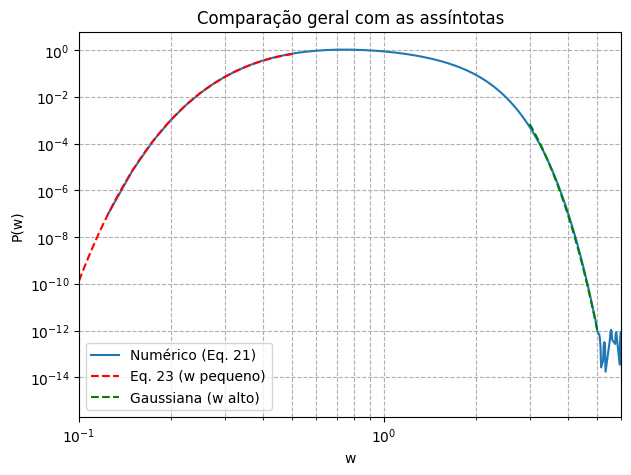
\includegraphics[scale=0.75]{colado14.png}
\par\end{center}

\bibliographystyle{plain}
\bibliography{tese,Artigo1/references,Artigo2/referencias,Artigo3/referencias}

\end{document}
